%
%  THESISBOEK
%
%  Dit bestand zorgt voor algemene (layout)definities, en groepeert de
%  afzonderlijke LaTeX-files tot een geheel.
%
%  @author Erwin Six, David De Reu, Brecht Vermeulen
%

\documentclass[11pt,a4paper,oneside,notitlepage]{book}
\usepackage[english]{babel}
\usepackage{algorithmic}
\usepackage{algorithm}
\usepackage{amsthm}
\usepackage{hyperref}
\usepackage{array}
%\usepackage[nottoc]{tocbibind} % Bibliografie in ToC; zie tocbibind.dvi

% marges aanpassen
% (opmerking: moet *voor* inclusie van fancyhdr package komen)
\setlength{\hoffset}{-1in}
\setlength{\voffset}{-1in}
\setlength{\topmargin}{2cm}
\setlength{\headheight}{0.5cm}
\setlength{\headsep}{1cm}
\setlength{\oddsidemargin}{3.5cm}
\setlength{\evensidemargin}{3.5cm}
\setlength{\textwidth}{16cm}
\setlength{\textheight}{23.3cm}
\setlength{\footskip}{1.5cm}

\usepackage{fancyhdr}
\usepackage{graphicx}
% \usepackage[colorlinks]{hyperref}
% Het bibliografisch opmaak bestand.
\bibliographystyle{unsrt}
%\bibliographystyle{bibliodutch}
%\bibpunct{[}{]}{,}{n}{,}{,}

\newtheorem{mydef}{Definition}

\pagestyle{fancy}

\renewcommand{\chaptermark}[1]{\markright{\MakeUppercase{#1}}}
\renewcommand{\sectionmark}[1]{\markright{\thesection~#1}}

\newcommand{\headerfmt}[1]{\textsl{\textsf{#1}}}
\newcommand{\headerfmtpage}[1]{\textsf{#1}}

\fancyhf{}
\fancyhead[LE,RO]{\headerfmtpage{\thepage}}
\fancyhead[LO]{\headerfmt{\rightmark}}
\fancyhead[RE]{\headerfmt{\leftmark}}
\renewcommand{\headrulewidth}{0.5pt}
\renewcommand{\footrulewidth}{0pt}

\fancypagestyle{plain}{ % eerste bladzijde van een hoofdstuk
  \fancyhf{}
  \fancyhead[LE,RO]{\headerfmtpage{\thepage}}
  \fancyhead[LO]{\headerfmt{\rightmark}}
  \fancyhead[RE]{\headerfmt{\leftmark}}
  \renewcommand{\headrulewidth}{0.5pt}
  \renewcommand{\footrulewidth}{0pt}
}

% anderhalve interlinie (opm: titelblad gaat uit van 1.5)
\renewcommand{\baselinestretch}{1.5}

% indien LaTeX niet goed splitst, neem je woord hierin op, of evt om splitsen 
% te voorkomen
\hyphenation{ditmagnooitgesplitstworden dit-woord-splitst-hier}

\begin{document}

%!!!!!!!!!!!!!!!!!!!!!!!!!!!!!!!!!!!!!!!!!!!!!!!!!!!!!!!!!!!!!!!!!!!!!!!!!!!!!!!!!!!!!!!!!!!!!!!!!
%!!!!!!!!!!!              onderaan/bovenaan elk blad thesistitel zetten                !!!!!!!!!!!
%!!!!!!!!!!!!!!!!!!!!!!!!!!!!!!!!!!!!!!!!!!!!!!!!!!!!!!!!!!!!!!!!!!!!!!!!!!!!!!!!!!!!!!!!!!!!!!!!!

% overzicht/samenvatting
%%  Overzichtsbladzijde met samenvatting

\newpage

{
\setlength{\baselineskip}{32pt}
\setlength{\parindent}{0pt}
\setlength{\parskip}{18pt}

\begin{center}

\noindent \textbf{\huge
Identifying experts through }
\textbf{\huge a framework for knowledge extraction}
\textbf{\huge from public online sources}

\setlength{\baselineskip}{12pt}
\setlength{\parindent}{0pt}
\setlength{\parskip}{12pt}

door 

Simon Buelens, Mattias Putman

Promotors: Prof.~Dr.~Ir.~Filip~De~Turck,~Elena~Tsiporkova~(Sirris),~Tom~Tourw\'{e}~(Sirris)\\
Scriptiebegeleiders: Anna~Hristoskova,~Tim~Wauters\\

Masterproef ingediend tot het behalen van de academische graad van\\
Master in de ingenieurswetenschappen: computerwetenschappen

Academiejaar 2010-2011\\
Faculteit Ingenieurswetenschappen\\
Voorzitter: Prof. Dr. Ir. Dani\"{e}l De Zutter\\
Vakgroep Informatietechnologie\\

\end{center}

\setlength{\baselineskip}{10pt}
\setlength{\parindent}{0pt}
\setlength{\parskip}{10pt}

\renewcommand{\baselinestretch}{1.1} 	% De interlinie afstand wat vergroten.
\small\normalsize                       % Nodig om de baselinestretch goed te krijgen.

\section*{Samenvatting}

Onderzoekers verliezen veel tijd met de zoektocht naar informatie gerelateerd aan hun onderzoeksdomein. Er bestaan bijna geen diensten die toelaten om aan de hand van trefwoorden een overzicht te verkrijgen met experts voor de opgegeven domeinen. Er is onderzoek naar disambiguatie van auteurs, maar deze worden meestal niet in combinatie gebracht met het opzoeken van experten, maar het indelen van publicaties (alhoewel de twee gerelateerd zijn).

In deze masterproef onderzoeken we de mogelijkheid om een framework op te stellen dat dit toelaat door online informatie op te zoeken, deze informatie in relatie te brengen met de correcte auteurs en gebruikers toe te laten dit framework te gebruiken om hierin te zoeken. De nadruk van het framework ligt op de disambiguatie van auteurs (aan de hand van de aanwezige informatie alle namen zo goed mogelijk connecteren met de juist auteur) aan de hand van een regelgebaseerde aanpak en de uitbreidbaarheid van het framework.

We maken gebruik van een graafgebaseerde representatie van de data en de architectuur is gebaseerd op pipes en filters. Dit laat toe dat het framework uitbreidbaar, schaalbaar en eenvoudig aanpasbaar is. Op het einde volgen de resultaten gebaseerd op een manueel geannoteerde testset. Uiteindelijk gaan we ook de vergelijking aan met de verdeling van auteurs door DBLP.

\section*{Trefwoorden}

auteur disambiguatie, data verwerking, clustering, pipes en filters

}

\newpage % strikt noodzakelijk om een header op deze blz. te vermijden


\pagestyle{fancy}
\frontmatter

% hoofdstukken
\mainmatter

\chapter{Framework Evaluation and Results}
\label{results}


We need to evaluate the performance of the framework. We will mainly focus our tests on the clustering of authors and the influence of different combinations of rules and parameters on the results. Proper clustering results in a collection of publications related to one author, allowing to define specialties and the level of expertise. 

In order to accomplish realistic and useful results, it's important the tests resemble realistic use-cases. This means testing against both general and borderline queries. Parameters making it easier in disambiguation are rare and country specific author names, a multitude of publications which are written with the same co-authors or the inclusion of the same email address. A combination of these parameters allows for easier manual checking of results, but is consequently less challenging. 

Borderline cases make more defiant evaluations. Author names containing foreign characters or accents make it easier to be misspelled. In contrast, common last names also make it harder to differentiate between different authors. Examples are Anderson or Smith in United States, Chen or Lee in East Asian countries or Peters in Belgium.

% Wat moeten we bespreken in dit hoofdstuk:

% De testopstelling
	% Hoe zit deze in elkaar
	% Waarom hebben hiervoor gekozen
	% Vergelijking met anderen?
% De bekomen resultaten
% (Vergelijken met andere mensen)

% Moeten we dit doen voor de clustering (dus vooral kijken naar name disambiguation) en de expert finding (hiervoor hebben we voornamelijk de category builder nodig voor goede resultaten)

\section{Evaluation Setup}

\subsection{Comparative Research}

The authors of \cite{han2004two} focus on disambiguating between authors having the same name or names which are very closely related. They use a dataset consisting of nine different names, each having at least 10 different name variations. For each variation they have collected publications from DBLP. An overview of this dataset can be viewed on \autoref{tab:auth-dblp-dataset} together with the results they achieve using different rules for disambiguation. The mean accuracy they accomplish with their best approach is $73.3\%$ with a standard deviation of $5.4\%$.

\begin{table}
	\centering
		\begin{tabular}[ht]{|c||c|c|c|c|c|c|}
			\hline
			\bfseries{Name} & \bfseries{Variations} & \bfseries{Size} & \bfseries{Coauthor} & \bfseries{Paper} & \bfseries{Journal} & \bfseries{Combination} \\
			\hline
			S Lee & 35 & 244 & 61.3\% & 14.3\% & 43.8\% & 65.4\% \\
			\hline
			J Lee & 33 & 172 & 70.9\% & 17.7\% & 39.9\% & 75.9\% \\
			\hline
			J Kim & 25 & 127 & 57.1\% & 18.8\% & 40.2\% & 66.1\% \\
			\hline
			Y Chen & 24 & 108 & 78.5\% & 14.0\% & 26.9\% & 81.7\% \\
			\hline
			S Kim & 20 & 94 & 69.0\% & 13.8\% & 27.6\% & 70.1\% \\
			\hline
			C Lee & 18 & 80 & 72.2\% & 13.9\% & 43.1\% & 75.0\% \\
			\hline
			A Gupta & 16 & 172 & 75.0\% & 25.6\% & 50.6\% & 78.1\% \\
			\hline
			J Chen & 13 & 91 & 66.3\% & 31.3\% & 44.6\% & 72.3\% \\
			\hline
			H Kim & 11 & 63 & 73.7\% & 21.1\% & 43.9\% & 75.4\% \\
			\hline
			\hline
			\bfseries{Mean} & & & 69.3\% & 18.9\% & 40.0\% & \bfseries{73.3\%} \\
			\hline
			\bfseries{StdDev} & & & 6.8\% & 6.1\% & 7.9\% & 5.4\% \\
			\hline
		\end{tabular}
	\caption{The nine DBLP datasets used in \cite{han2004two}. Each row contains the base name, the number of recorded variations and the total amount of examined publications of this name. The last four columns show the accuracy measured using the different rules. The two bottom rows give the mean accuracy for the rules and the standard deviation.}
	\label{tab:auth-dblp-dataset}
\end{table}

It is important to note that the division of the clusters is solely based on the division of the authors in DBLP. As this division on DBLP is often wrong, we find that this makes a poor benchmark. Getting very high accuracy when comparing to DBLP does not mean the result is good. In order to get a proper insight into the disambiguation quality, we would still have to check the results manually. This is the main reason we choose to compose our own dataset.

\subsection{Test Set}
\label{sec:testset}

As stated before, we want to resemble a realistic combination of easier and harder use-cases for our own dataset. As \autoref{tab:testset} shows, we have chosen five base names, each with a number of variations and have manually disambiguated these variations and combined the authors into clusters using the information on DBLP and the actual papers, if they were available. In total our test set contains just over a 1000 publications. An overview of the names that correspond to each of these base names, can be found in \autoref{appendix:dataset}, together with links to DBLP. In order to make it easier, we will use the following definition in the rest of the text:

\begin{mydef}
	\bfseries{Family} With the term family, we refer to one of the five base names.
\end{mydef}

Nevertheless we composed the clusters manually, there are no guarantees that this is completely accurate. Especially for the families "Chen" and "Johnson", there might be small mistakes as the amount of different authors is overwhelming. However, the dataset we composed is a lot more accurate than DBLP. The comparison between the number of authors represented by DBLP and the number of authors we disambiguated, is also shown on \autoref{tab:testset}.

\begin{table}
	\centering
		\begin{tabular}[ht]{|c|c|c|c|}
			\hline
			\bfseries{Name Set} & \bfseries{Authors} & \bfseries{Publications} & \bfseries{DBLP} \\
			\hline
			Turck & 4 & 172 & 4 \\
			\hline
			Chen & 70 & 221 & 1 \\
			\hline
			Woo & 1 & 9 & 3 \\
			\hline
			Mens & 2 & 153 & 2 \\
			\hline
			Johnson & 107 & 460 & 64 \\
			\hline
		\end{tabular}
	\caption{The classification of our manually composed dataset. The first column contains the family. This is the name we used to find the authors on DBLP. The second column gives the number of clusters we defined manually for this family. The third column gives the number of publications we found on DBLP and the last column gives the number of different authors DBLP gives for this base name.}
	\label{tab:testset}
\end{table}

In order to be able to test the affiliation and the email rule, we had to get affiliations and email addresses for each of the authors of each publication. We started with writing a new pipe that would be able to search the publication on Bing \cite{bing}. The amount of papers that are actually available on Bing is abysmal, rendering this pipe useless. As the focus of our thesis is information processing, rather than retrieval, we manually added the affiliation and the email address of the author we are examining to each of the publications, if we could find them. This allows us to still test the rules.

\subsection{Setup}

A simplified overview of the test setup is shown in \autoref{fig:testsetup}. We start with the links of the author of a family we want to add. This is the input for the framework. The framework will search publications on DBLP for each of this link and combine them with the email and affiliation information that have been composed manually. The result is a graph containing clusters with the different authors. We extract the clusters from the graph and pass them to the result calculator. This is a script that calculates the precision, recall and $F_{1}$ measure by comparing the calculated clusters with the manually composed dataset, as explained in \autoref{sec:testset}, which is called the "ground truth" in \autoref{fig:testsetup}.

\begin{figure}[htb]
	\centering
		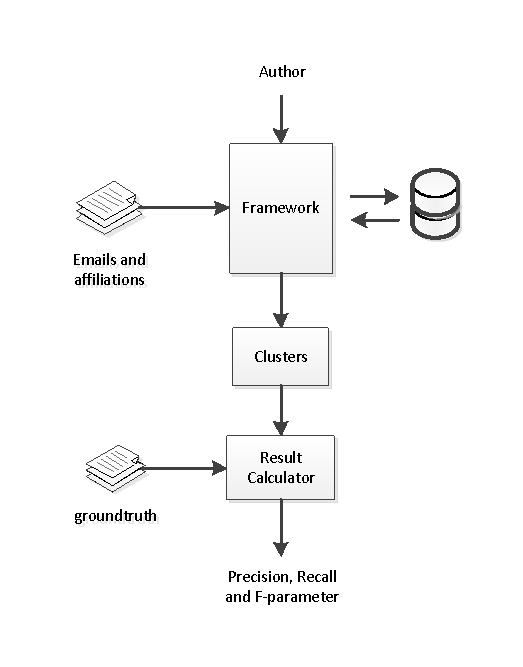
\includegraphics{./fig/testsetup.pdf}
	\label{fig:testsetup}
	\caption{A simplified overview of the test setup starting with the author name and ending with the accuracy results.}
\end{figure}

The result calculator calculates the precision, recall and F measure as defined in \autoref{eq:prf}. Unless explicitly stated otherwise, when we refer to F measure, we mean the $F_{1}$ measure where recall and precision are equally important. These statistical values are calculated for each of the clusters from the ground truth. 

\begin{equation}
	\label{eq:prf}
	\begin{array}{r c l}
		precision & = & \frac{\left|\left\{relevant~documents\right\} \cap \left\{retrieved~documents\right\}\right|}{\left|\left\{retrieved~documents\right\}\right|} \\
		recall & = & \frac{\left|\left\{relevant~documents\right\} \cap \left\{retrieved~documents\right\}\right|}{\left|\left\{relevant~documents\right\}\right|} \\
		F_{\beta} & = & ( 1 + \beta^{2} ) * \frac{precision * recall}{\beta^{2} * precision + recall} \\
	\end{array}
\end{equation}

If we denote the cluster of the ground truth as $C_g$, then the calculated cluster from the graph the result calculator will $C_g$ compare with is given by 

\begin{equation}
	\label{eq:calccluster}
	\min_{\forall c \in calculated~clusters}{\left| C_g \setminus c \right|}
\end{equation}

In \autoref{eq:prf}, we use the terms relevant and retrieved documents. The explanations of these terms are given by the following definitions.

\begin{mydef}
	\textbf{Relevant documents} The publications from the cluster in the ground truth.
\end{mydef}

\begin{mydef}
	\textbf{Retrieved documents} The publications from the cluster calculated by the framework belonging to the cluster in the ground truth, calculated in \autoref{eq:calccluster}.
\end{mydef}

After calculating these statistical values for all the clusters in the ground truth, the mean F measure is calculated to give us an idea of the accuracy for a given test.

\section{Results}

\subsection{Synchronous versus Asynchronous Execution}

Any connection in a pipe network can be configured to be local or asynchronous. Asynchronous connections push the flow in a shared queue of flows that need to be processed. A pool of workers on different machines will poll this queue and resume the flow on their own machines, making the pipe network distributed. We expect this scaling to entail an increase in performance.

We notice that a pipe network that is executed synchronously spends more than 50\% of its time waiting for input. This is because accessing websites, distributed memory or the graph is associated with a certain latency causing pipes to wait for the service to respond. The amount of time spent waiting heavily depends on the characteristics of the input and the hardware. Some inputs require more computation and others more communication. When we run three workers on the same machine, we can already perceive a speedup of 200-300\%.

We expect that distributing the pipes over multiple servers would have a enormous impact on performance. The pipes try to minimize the amount of communication with the graph database as much as possible, making the system more scalable. As we do not have decent server hardware at our disposal, we were not able to test this.

\subsection{Rules}

We have tested the influence of the different rules on the accuracy. For each of the families, we tested the same combination of rules in succession. The F measure for each of these combinations can be seen on \autoref{fig:test-rules}. The combination of all four rules, renders the best result, although sometimes the increase in accuracy from an additional rule is minimal. For "Chen", adding the affiliation rule to the community and email rule even results in a small decrease in accuracy. This is because certain authors are clustered together wrongly. The exact F measures for this combination can be found in \autoref{tab:comparison-dblp}. 

\begin{figure}[htb]
	\centering
		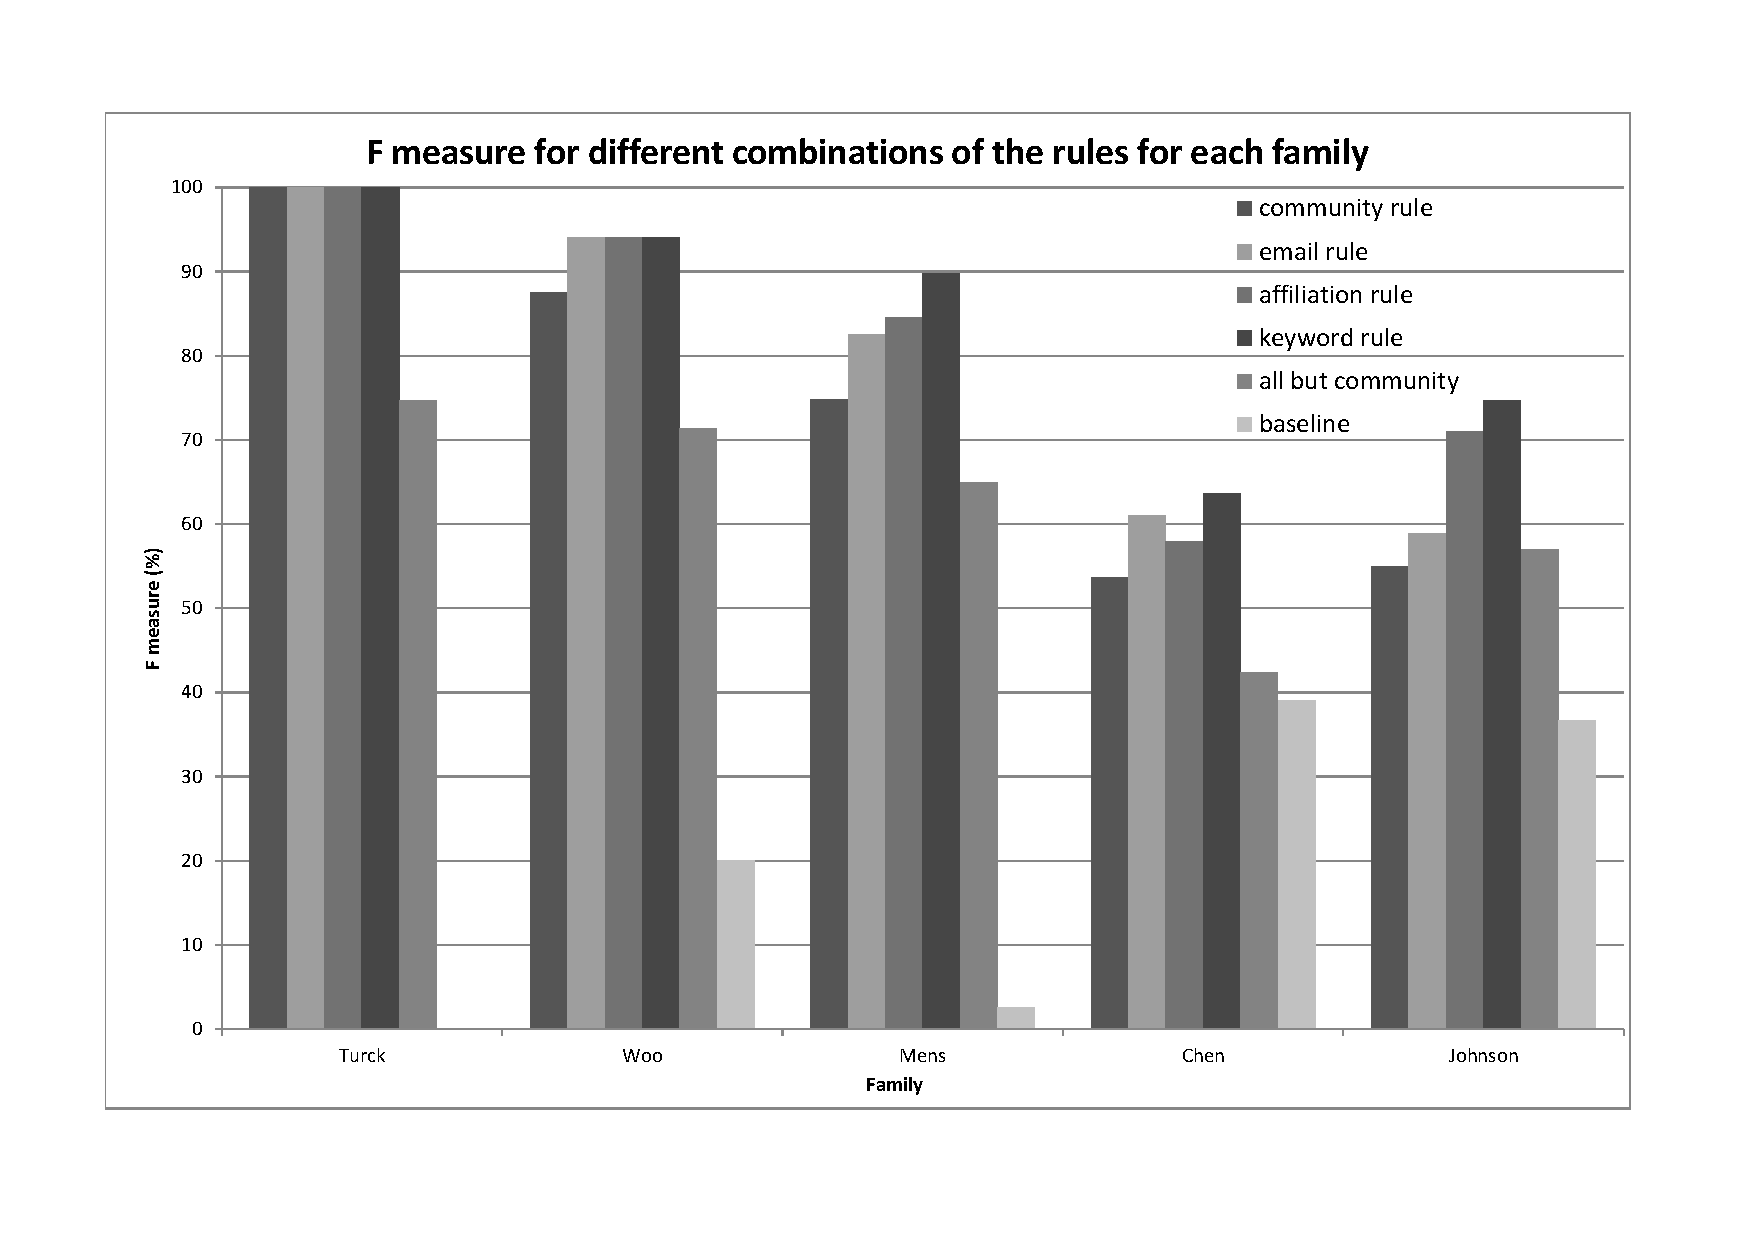
\includegraphics[width=0.80\textwidth]{./fig/test-rules.pdf}
	\caption{A comparison of the accuracy, measured as F score, for the different rules and combinations. The first column shows the use of just the community rule (community rule). The second column shows it in combination with the email rule (email rule). The third rule is a combination of the previous two with the affiliation rule (affiliation rule), while the fourth is a combination of all four rules (keyword rule). The fifth column shows the combination of the email, affilation and keyword rule. The last column gives the so-called baseline, this is the F measure we get when all authors are considered different authors.}
	\label{fig:test-rules}
\end{figure}

The weights we used for the different rules are the same in each of the tests and is the result of \autoref{sub:weights}. We used the weight distribution called "highkey", as denoted in \autoref{table:highkey}, as this distribution yielded the highest average accuracy.


% bespreek figuur

\subsection{Weights}
\label{sub:weights}

We have tested different values for the weights allocated to each of the rules and also the value of $\alpha$ which is used to determine if reclustering should occur. The results are shown on \autoref{fig:test-weights}, while the different distributions are depicted in \autoref{table:distributions}. The average F measure for each distribution over the five families is given by:

\begin{table}[ht]
	\center
	\begin{tabular}{|c|c|}
		\hline
		\bfseries{Distribution} & \bfseries{Average F measure} \\
		\hline
		basic & 81,5\% \\
		\hline
		lowkey & 72,7\% \\
		\hline
		highco & 79,0\% \\
		\hline
		highkey & 84,5\% \\
		\hline
	\end{tabular}
	\caption{The average F measure over the five families for each of the weight distributions.}
	\label{tab:avg-f-distr}
\end{table}

The distribution "highkey" gets the best average accuracy. This distribution gives high values to all properties, favoring a lot of clustering, while the higher alpha makes sure there is still a threshold. Only for family "Johnson", it doesn't get the highest F measure. This can be attributed to too much clustering, resulting in a higher recall, but a lower precision. The actual F measures for this distribution can be seen in \autoref{tab:comparison-dblp}.

\begin{table}[ht]
	\begin{minipage}[b]{0.5\linewidth}\centering
		\begin{tabular}{|c|c|}
			\hline
			\bfseries{Property} & \bfseries{Weight} \\
			\hline
			$\alpha$ & 25 \\
			\hline
			keyword rule & 4\\
			\hline
			community rule & 8\\
			\hline
			affiliation rule & 10\\
			\hline
			email rule & 1000\\
			\hline
		\end{tabular}
		\caption{Basic}
	\end{minipage}
	\begin{minipage}[b]{0.5\linewidth}
		\centering
		\begin{tabular}{|c|c|}
			\hline
			\bfseries{Property} & \bfseries{Weight} \\
			\hline
			$\alpha$ & 25 \\
			\hline
			keyword rule & 1\\
			\hline
			community rule & 8\\
			\hline
			affiliation rule & 10\\
			\hline
			email rule & 1000\\
			\hline
		\end{tabular}
		\caption{Lowkey}
	\end{minipage}
	\begin{minipage}[b]{0.5\linewidth}\centering
		\begin{tabular}{|c|c|}
			\hline
			\bfseries{Property} & \bfseries{Weight} \\
			\hline
			$\alpha$ & 25 \\
			\hline
			keyword rule & 1\\
			\hline
			community rule & 50\\
			\hline
			affiliation rule & 10\\
			\hline
			email rule & 1000\\
			\hline
		\end{tabular}
		\caption{Highco}
	\end{minipage}
	\begin{minipage}[b]{0.5\linewidth}
		\centering
		\begin{tabular}{|c|c|}
			\hline
			\bfseries{Property} & \bfseries{Weight} \\
			\hline
			$\alpha$ & 25 \\
			\hline
			keyword rule & 10\\
			\hline
			community rule & 50\\
			\hline
			affiliation rule & 10\\
			\hline
			email rule & 1000\\
			\hline
		\end{tabular}
		\caption{Highkey}
		\label{table:highkey}
	\end{minipage}
	\caption{Weight distributions with the name of each distribution as used in \autoref{fig:test-weights}}
	\label{table:distributions}
\end{table}

\begin{figure}[htb]
	\centering
		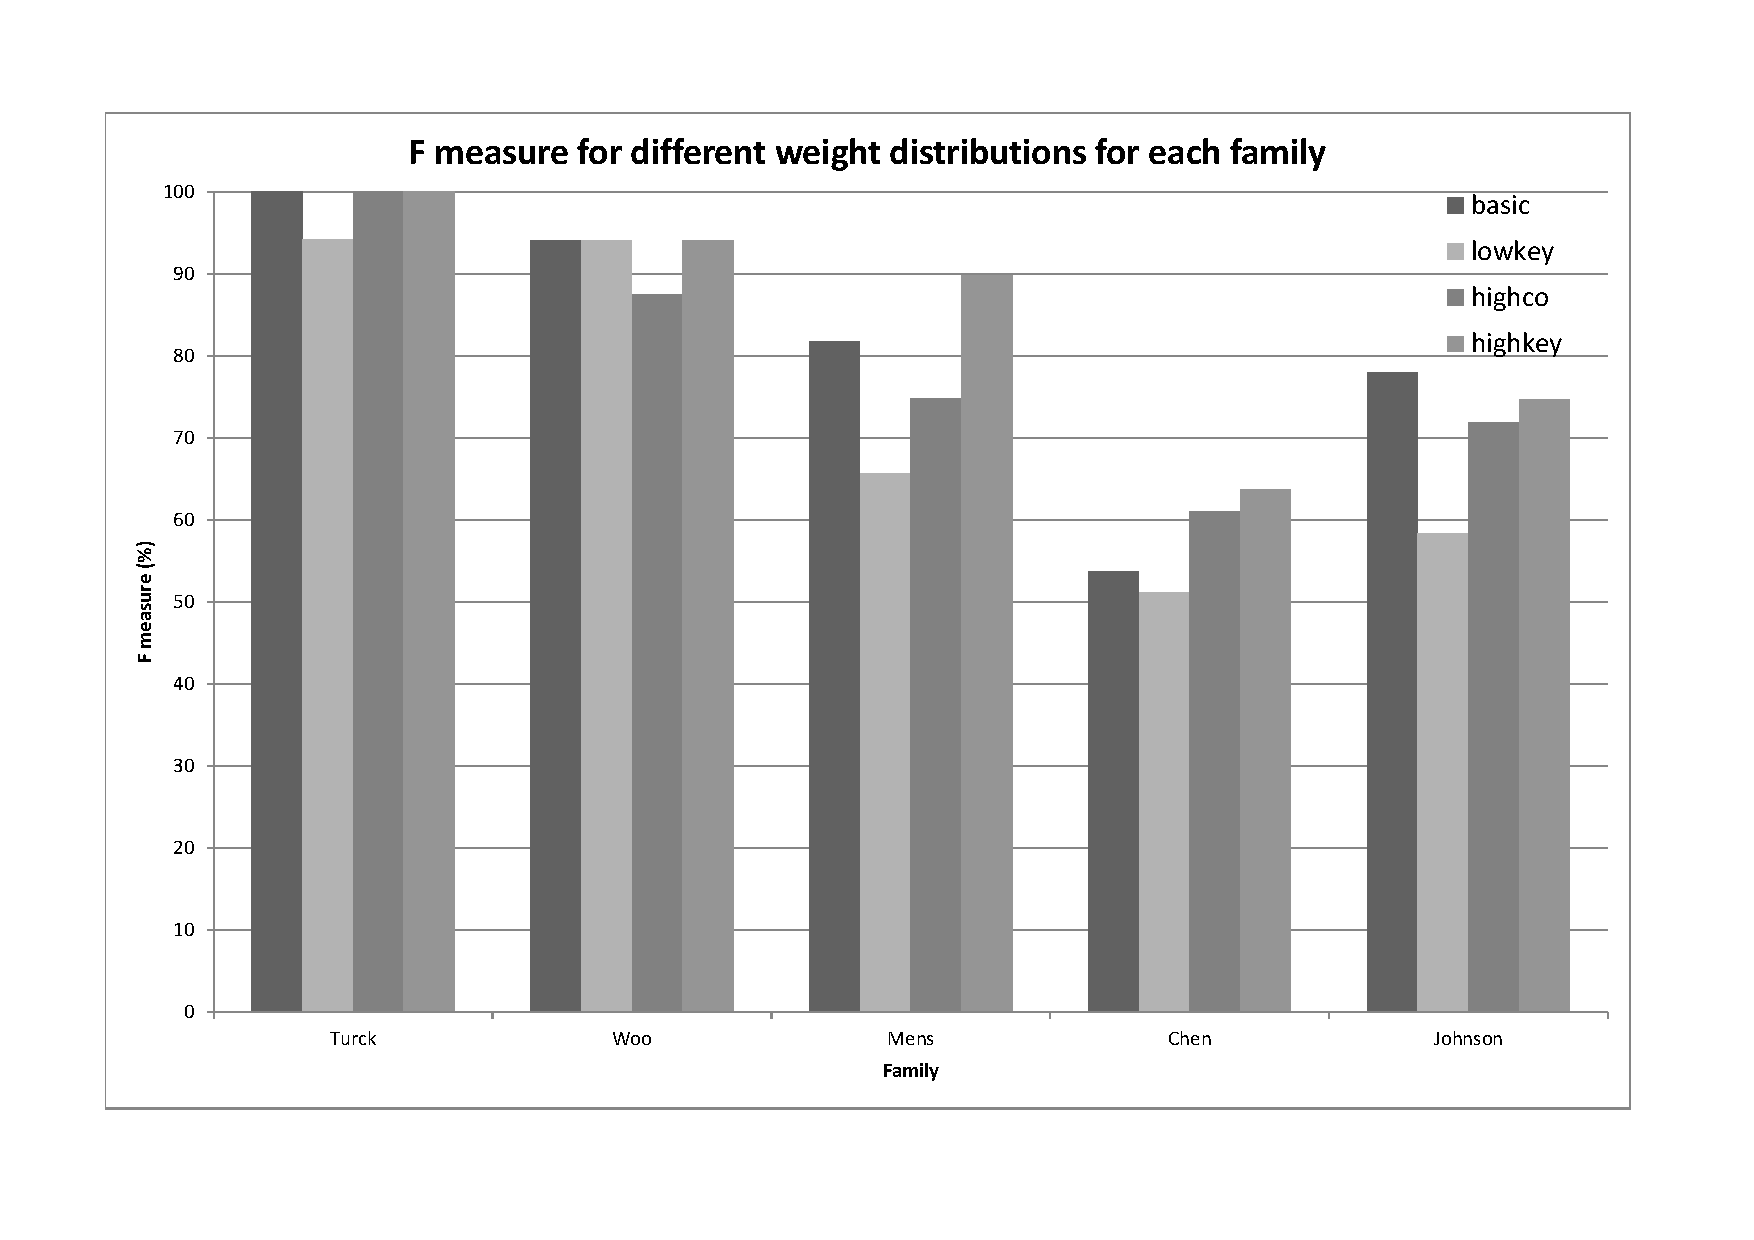
\includegraphics[width=0.80\textwidth]{./fig/test-weights.pdf}
	\caption{The F measure for different weight distributions for each family. The weight distributions, from left to right, are "basic", "lowkey", "highco" and "highkey". The actual value for the distributions is shown on \autoref{tab:avg-f-distr}.}
	\label{fig:test-weights}
\end{figure}

\subsection{Comparing to DBLP}

We have calculated the F measure for each of the families as they are divided on DBLP, to make a comparison with our own results. The values are shown on \autoref{tab:comparison-dblp}. The divisions for "Turck" and "Mens" are completely correct, the other three are far less accurate with "Chen" having an astonishingly low F measure of $2.73\%$. We compare the F measure to our highest average scoring distribution, "highkey". We also compare the mean F measures and a weighted variation of the mean measure which is calculated using the following formula ($F_X(f)$ is the F measure for family name $f$ for $X$):

	\[
	\sum_{f \in families}{\frac{F_{X}(f)}{|f_{publications}} * N},~X \in \left\{DBLP,highkey\right\},~N = total~number~of~publications
\]

Our framework scores $14\%$ to $17\%$ better than DBLP, depending on how the mean value is measured.

\begin{table}
	\centering
		\begin{tabular}{|c|c|c|c|c|c|c|c|}
			\hline
			& \bfseries{Turck} & \bfseries{Woo} & \bfseries{Mens} & \bfseries{Chen} & \bfseries{Johnson} & \bfseries{Mean} & \bfseries{Weighted} \\
			\hline
			\bfseries{DBLP} & 100.0\% & 87.5\% & 100.0\% & 2.7\% & 62.8\% & 70.6\% & 61.8\% \\
			\hline
			\bfseries{Highkey} & 100.0\% & 94,1\% & 89,8\% & 63,7\% & 74,7\% & 84,5\% & 79,0\% \\
			\hline
		\end{tabular}
	\caption{Comparison of the F measures for the different families as they are divided on DBLP and as calculated by our framework. The last columns give the mean F measure and a weighted distribution based on the number of papers in each family.}
	\label{tab:comparison-dblp}
\end{table}
\backmatter
\end{document}
